\documentclass[11pt,a4paper]{article}
\usepackage{chngcntr}
\counterwithin{figure}{section}
\usepackage[T1]{fontenc} \usepackage{lmodern} \usepackage[utf8]{inputenc} \usepackage[english]{babel} \usepackage{amssymb} \usepackage{amsmath} \usepackage[round]{natbib} \usepackage{xcolor,graphicx}
\author{Zully Faralli, Marc Spörri} \title{Analysis and forecasting of the Swiss Tent Index Time Series, 1993 to 2018} \date{\today}
\begin{document}
\maketitle


\section{Introduction}
describe aims of your project and give an overview of the report. describe briefly the methods you have used to analyze the data.
\\
\\
copied from the proposal: The main goal of the project is to draw inference from the rent index time series and to predict their
future values and a future trend. In order to do that we have first to transform the data in a
stationary time series, either by fitting a polynomial trend, either by differencing. Afterwards we are
going to fit a model to our data. The model will be used to describe and interpret our data as well as
to predict future values.

\section{Data Description}
Describe the data and the context in which it has been gathered and explain. Give some general references about the data.
\\
\\
copied from the proposal: The data is provided by the Swiss Federal Statistical Office, implying 100 quarterly observations of
the Swiss rent index beginning by the 2nd quarter of the year 1993 and ending by the first quarter of
the year 2018. The rent index measures the inflation of the rented dwellings in Switzerland. It is the
most significant partial index of the Swiss consumer’s price index, representing a weighted share of
13 percent of this index. The data are collected quarterly, based upon a stratified random survey sampling
of around 10'000 lessors. The time series’ first observation (2nd quarter of the year 1993) will be the
reference value which is set to a base index of 100 and represents the weighted average rent at this
time in Switzerland (OFS, 2016: p. 20-23).

\section{Data Analysis and Transformation into a Stationary Time Series}
Describe your models carefully, give references, justify your choices. You can use the guidelines provided below.
\\1. Do you transform the data? If yes, give the transformation you used and explain this choice. 2. Does the series show a trend and a seasonality? 
\\If yes, describe how you model them. Check the plot of the residuals. 
\\3. Comment the autocorrelation and the partial autocorrelation of the residual series obtained after removing the trend and seasonality.
\\4. Model the residuals with an appropriate model. If you consider different models, explain strengths and weaknesses of each model.
\\5. Comment the diagnostig plots of the model(s) you chose. you can plot the standardized residuals, the normal qqplot, the ACF and PACF of the residuals, and the p-value of the Ljung-Box-Tests for different lags to assess stationarity, independence and normality of the residuals.
\\6. By means of your model, make some predictions and give confidence intervals for the prediction. you can illustrate it by showing some plots.
\\
\\
The first step in any analysis of a time series is to plot the data in order to identify discontinuities or a sudden change of level in the series (book p. 23). As we can see from figure~\ref{fig:indiceloyers_timeseries} there seems to be a clear positive trend. 
\\In addition it may be advisable as well to analyze the series by breaking it into homogeneous segments (book p.23) . Let's have a look at the segmented plots  1993 to 2009 and 2009 to 2018 in figure~\ref{fig:indiceloyers_test} and figure~\ref{fig:indiceloyers_train}. We can see a slightly slower increase in the segment from 2009 to 2018 indicating that in the years from 1993 to 2009 the growth in rental prices was higher than in the years in the second's segment which begins from 2009. that can be explained by the big baisse in the early 90ies, starting from a lower initial point and having better conjunctural perspectives the increase was stronger, whilst from 2009 on the growth in rental prices slowed down, which can be very well explained by the US subprime crises beginning in the year 2008 followed by a long-taking global recession. However they are no sudden changes in level or huge outliers, therefore we can start to find a transformation into a stationary time series for our whole data.
\begin{figure}
\centering
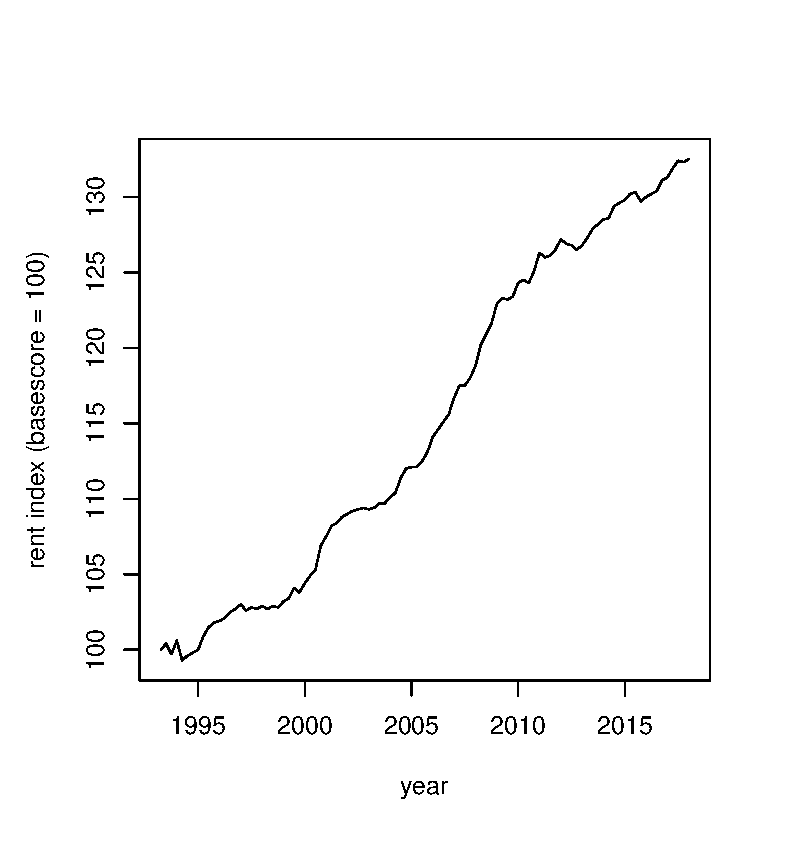
\includegraphics[angle=0,
width=0.7\textwidth]{indiceloyers_timeseries}
\caption{Swiss rent index, years 1993 to 2018\label{fig:indiceloyers_timeseries}}
\end{figure}
\begin{figure}
\centering
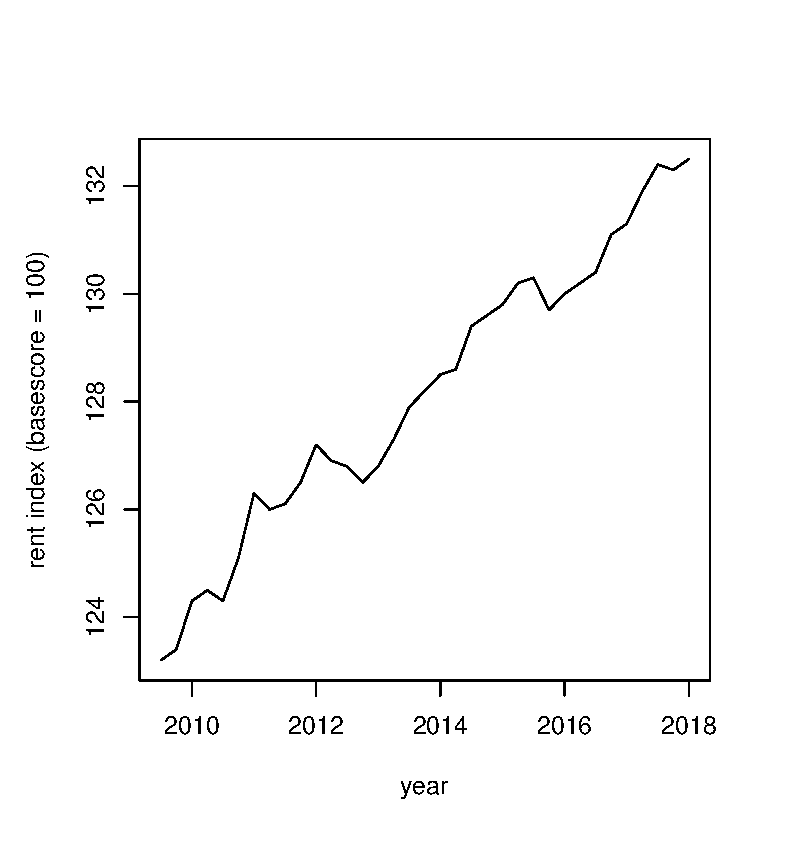
\includegraphics[angle=0,
width=0.7\textwidth]{indiceloyers_test}
\caption{Swiss rent index, years 2009 to 2018\label{fig:indiceloyers_test}}
\end{figure}
\begin{figure}
\centering
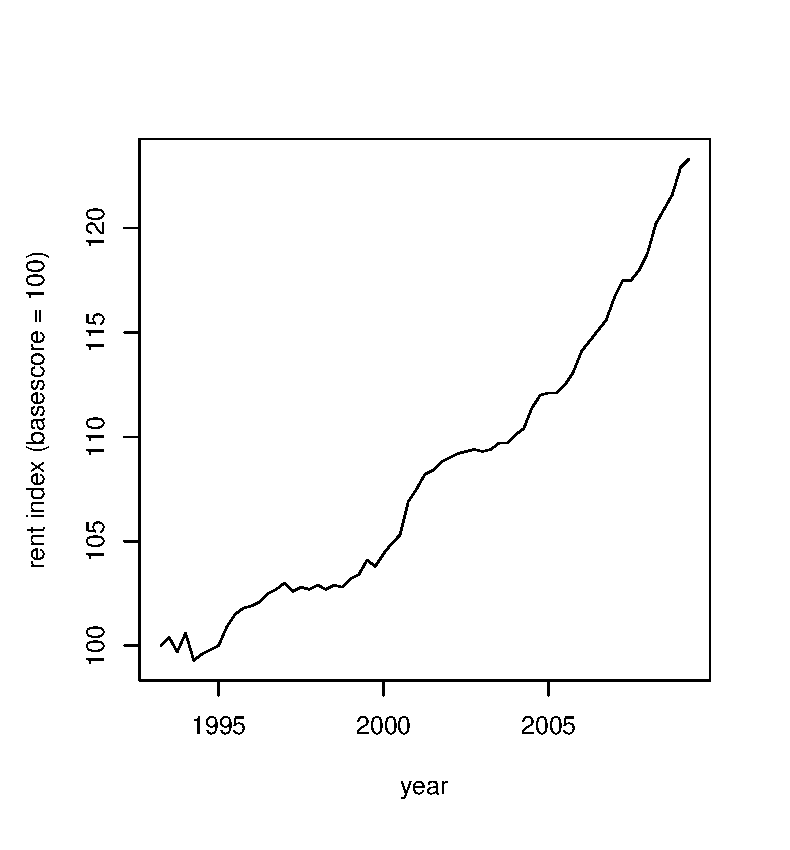
\includegraphics[angle=0,
width=0.7\textwidth]{indiceloyers_train}
\caption{Swiss Rent index, years 1993 to 2009\label{fig:indiceloyers_train}}
\end{figure}

To get a stationary time series, which means we want to generate a noise sequence whose covariances are not depending on time (book p. 35), we have to eliminate any trend and/or seasonal components in our data. A trend is obviously visible from figure~\ref{fig:indiceloyers_timeseries}, however we cannot be that sure if it doesn't exist a seasonal component either. Therefore in the next step we estimate a possible seasonal component by linear regression. 

\subsection{Check for Seasonality}
Since the data are collected quarterly we use a linear regression model with d=4 dummy predictors, ergo a dummy for every season (LN1-2, p. 36). 
\begin{figure}
\centering
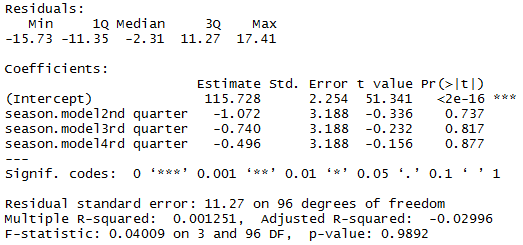
\includegraphics[angle=0,
width=0.7\textwidth]{summary_seasonmodel}
\caption{summary statistics of the fitted seasonal model\label{fig:summary_seasonmodel}}
\end{figure}
As we can see from figure~\ref{fig:summary_seasonmodel} none of the estimated seasonal coefficients are significant. We can be sure now that they are no seasonal impacts on our data, hence what remains is to eliminate the trend. In the absence of a seasonal component our model becomes the following (Brook Davis p. 24):
\begin{equation}
X_t = m_t + Y_t, \text{t = 1,...,n,} 
\\where EY_t = 0
\end{equation} 

\subsection{Trend Elimination by fitting polynomial models}
As we have shown above in order to model our data we don't have to get rid of seasonal components, nevertheless we have to get rid of the obvious trend. Whilst the time series \ref{fig:indiceloyers_timeseries} indicates a probable polynomial trend, especially a linear one, we are starting by fitting different polynomial trends by ordinary least squares estimation. We are fitting a linear trend, a quadratic trend, a cubic trend as well as a logarithmic trend. The latter  helps to transform a potentially exponential increase in the rent index into a linear trend, even though at first sight the time series \ref{fig:indiceloyers_timeseries} looks more like a linear than an exponential trend, we are going to test for a logarithmic trend either.
\\
\begin{figure}
\centering
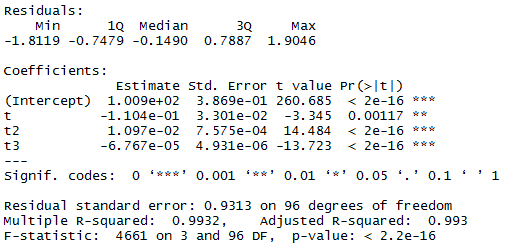
\includegraphics[angle=0,
width=0.7\textwidth]{summary_cubicmodel}
\caption{summary statistics of the fitted cubic model\label{fig:summary_cubicmodel}}
\end{figure}
The coefficients in all 4 models are highly significant and with an $R^2$-Value of 98 to 99 percent (meaning that the models would be able to explain up to 98percent (99percent respectively) of the variance), the linear, the quadratic and the cubic model would explain our data extremely well which can be well seen on the cubic model's example in \ref{fig:summary_cubicmodel}. The logarithmic model shows a bit less explanatory power with an $R^2$-Value of 0.72, even though its coefficient is highly significant as well. However we have to be careful with the interpretation of the p-values since this regression models assume independence of the observations whereas our purpose of the summary statistics of fitted linear models is a different one: to use regression in order to construct a stationary time series (Brooks Davis p. xy). 

\subsubsection{Diagnostics of the fitted polynomial trends}

\begin{figure}
\centering
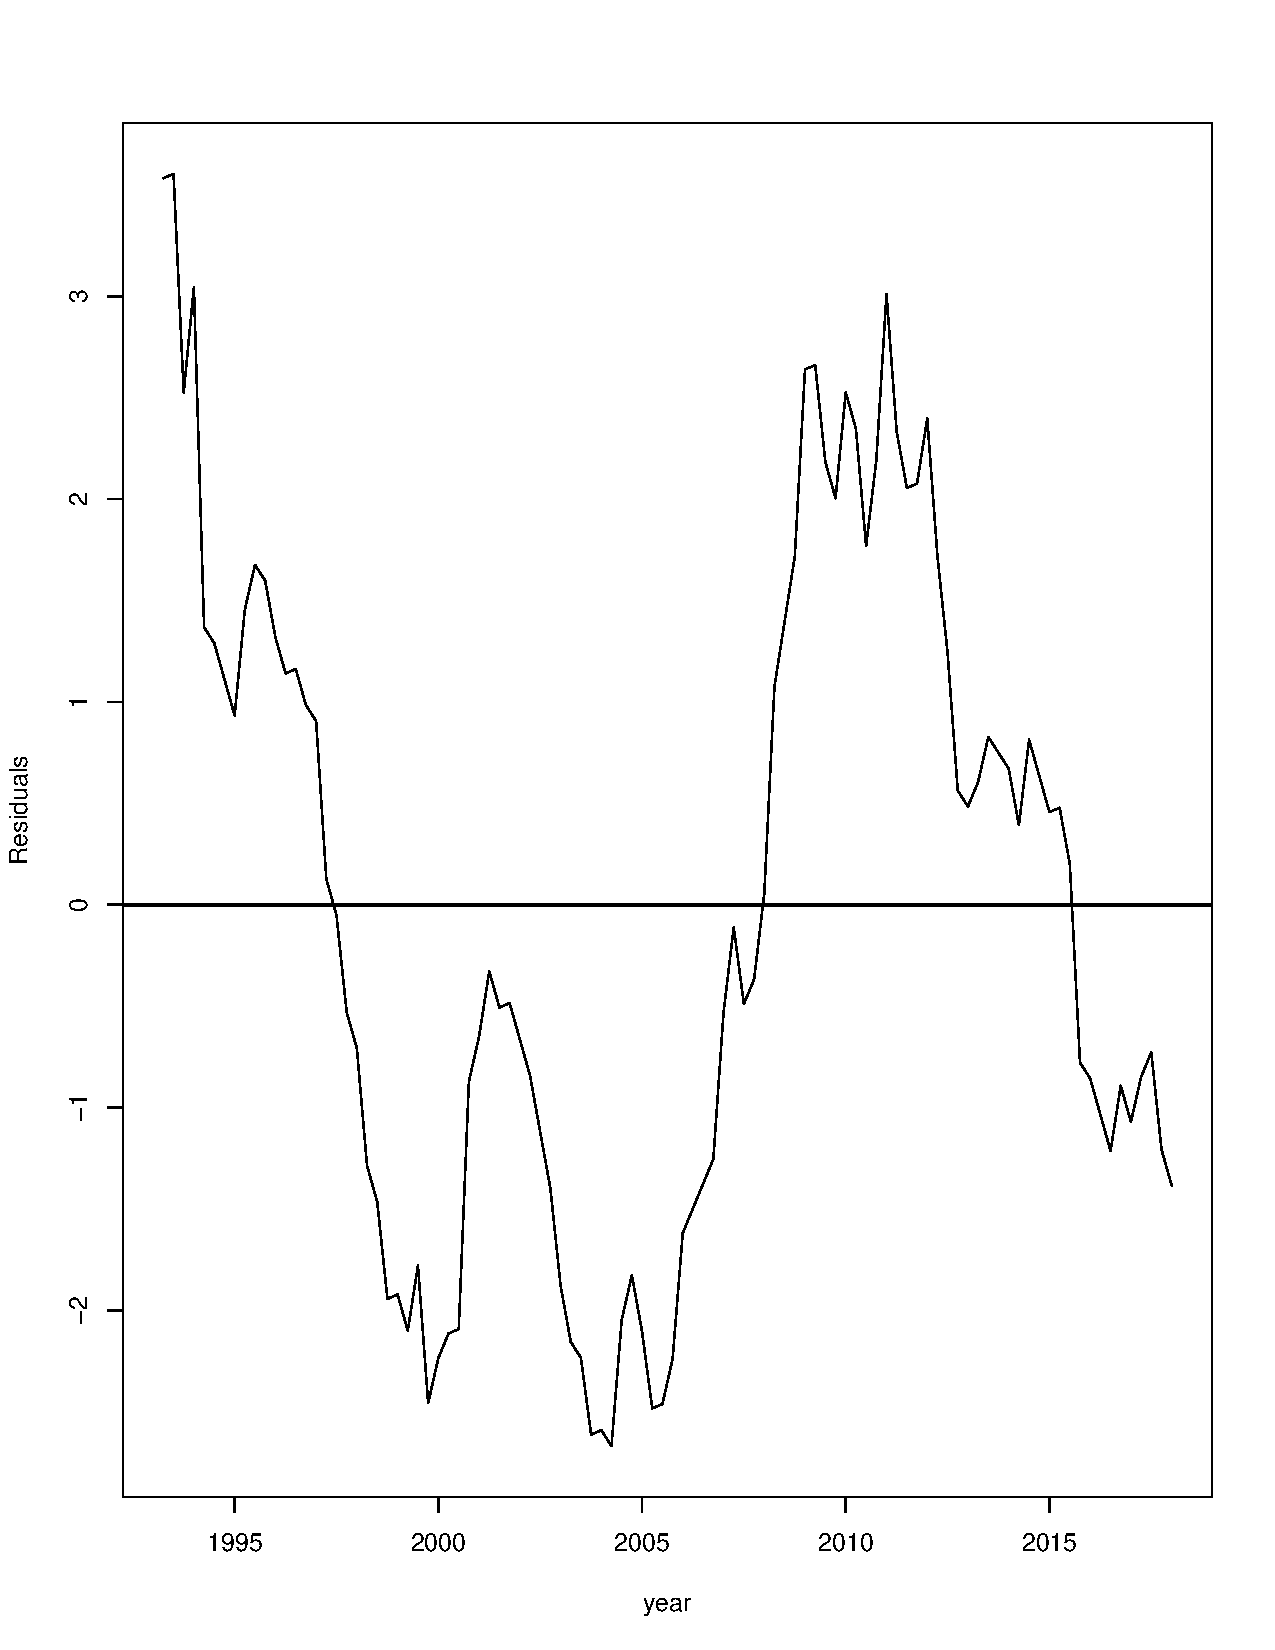
\includegraphics[angle=0,
width=0.5\textwidth]{resid_linearmodel}
\caption{Residuals of a fitted linear model
\label{fig:resid_linearmodel}}
\end{figure}

\begin{figure}
\centering
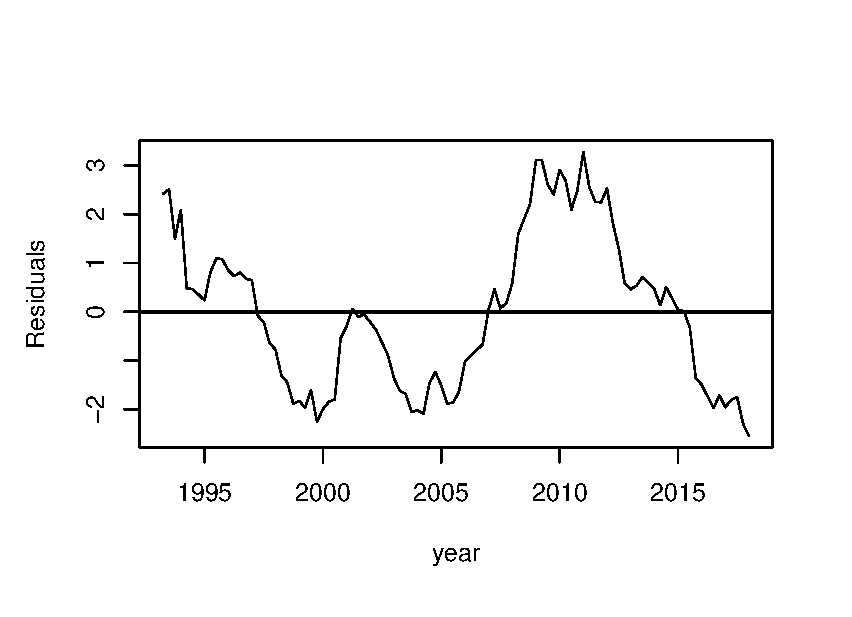
\includegraphics[angle=0,
width=0.5\textwidth]{resid_quadraticmodel}
\caption{Residuals of a fitted quadratic model
\label{fig:resid_quadraticmodel}}
\end{figure}

\begin{figure}
\centering
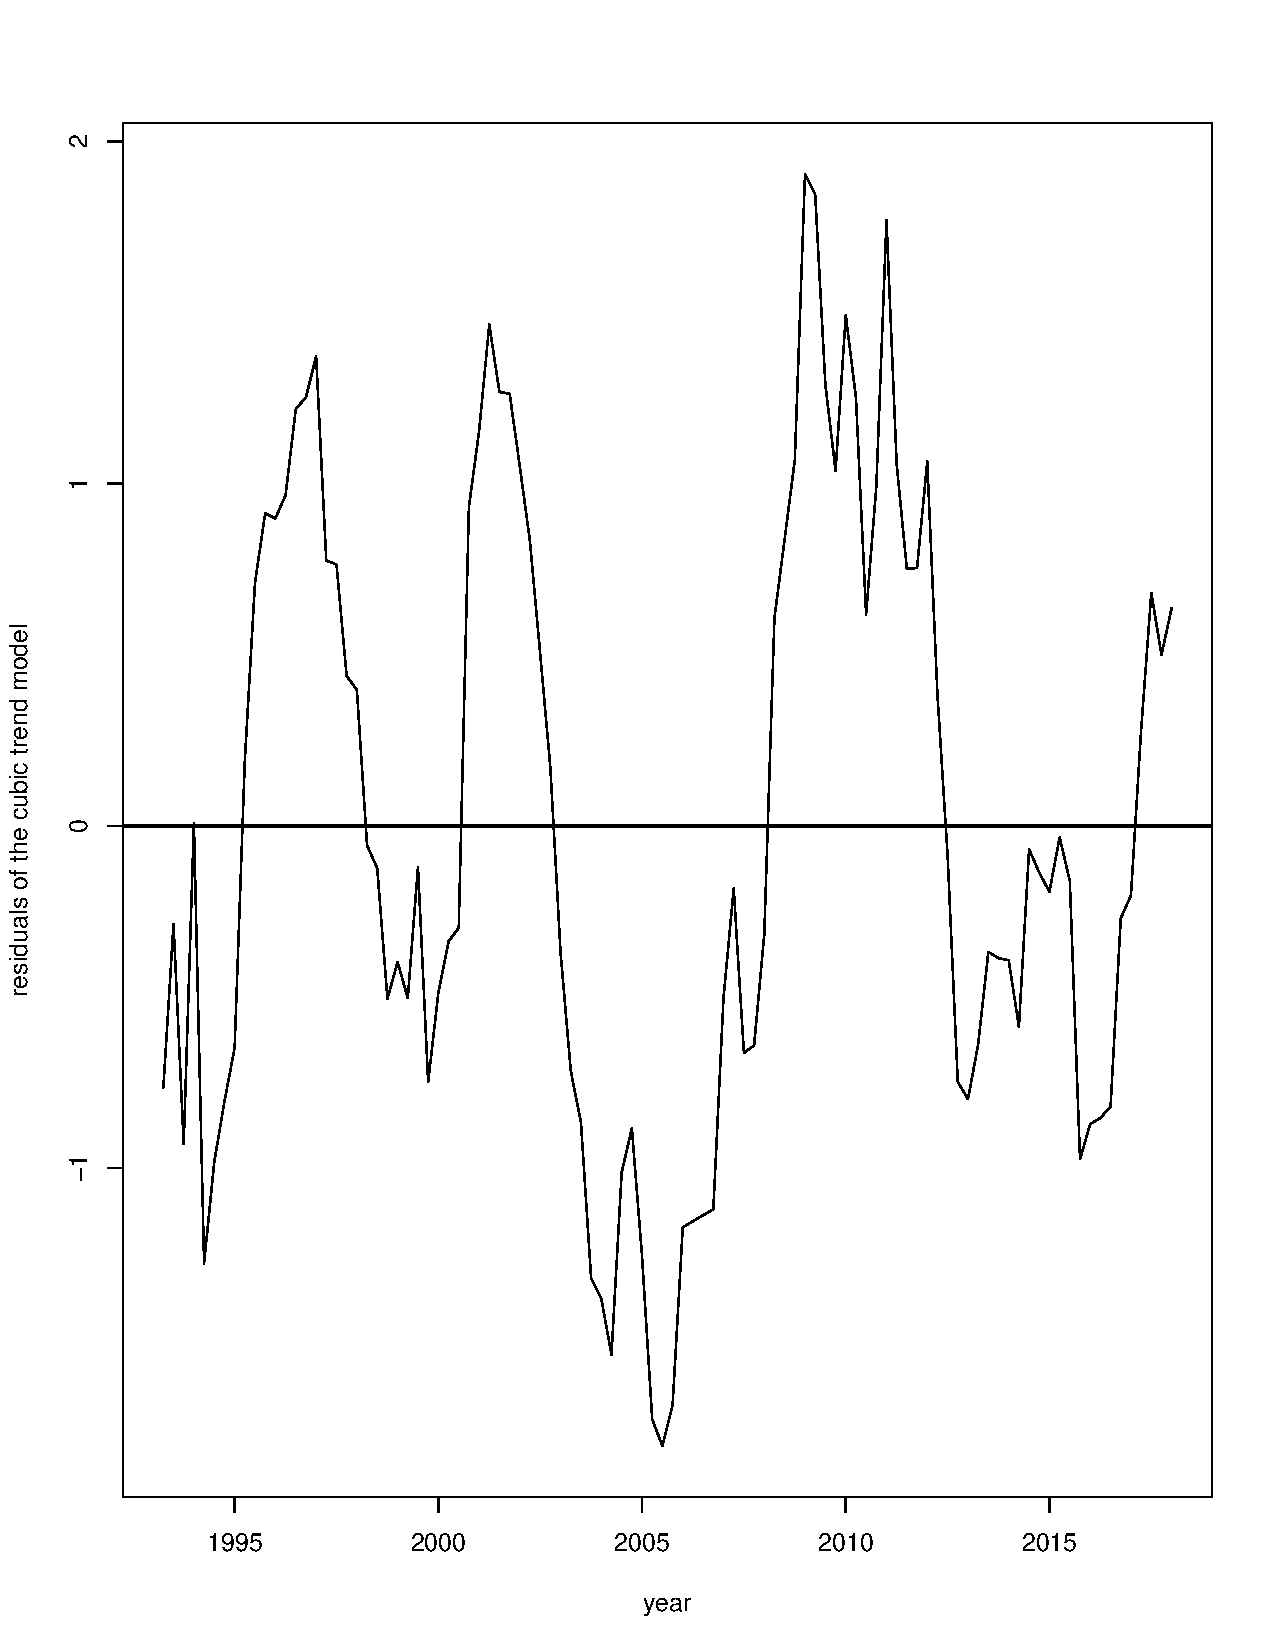
\includegraphics[angle=0,
width=0.5\textwidth]{resid_cubicmodel}
\caption{Residuals of a fitted cubic model
\label{fig:resid_cubicmodel}}
\end{figure}

\begin{figure}
\centering
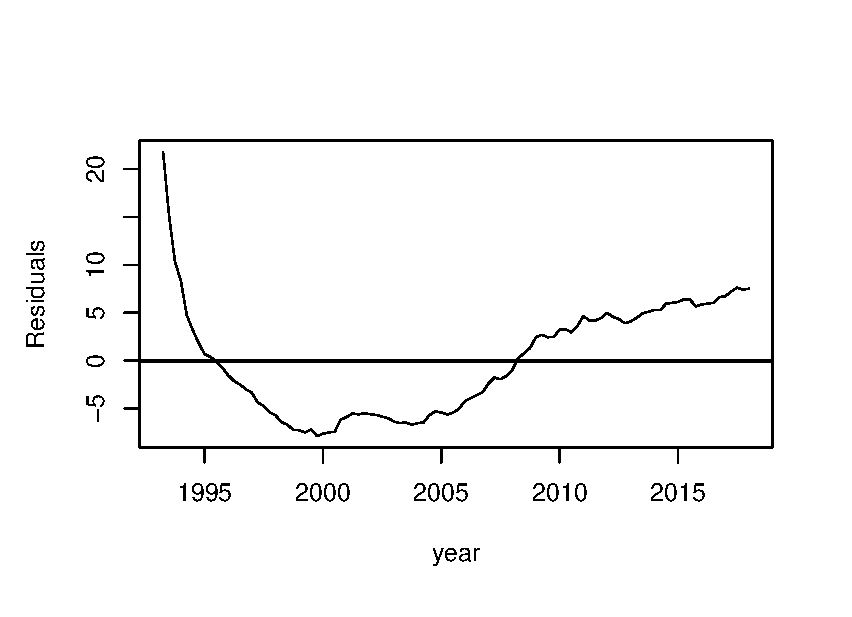
\includegraphics[angle=0,
width=0.5\textwidth]{resid_logmodel}
\caption{Residuals of a fitted logarithmic model
\label{fig:resid_logmodel}}
\end{figure}
Unfortunately the plots for polynomial trend elimination don't show any stationarity, as we can derive from the four figure~\ref{fig:resid_linearmodel}, figure~\ref{fig:resid_quadraticmodel}, figure~\ref{fig:resid_cubicmodel} and figure~\ref{fig:resid_logmodel}. The four plots show large covariances and their residuals are evidently depending on time $t$.
\\
\begin{figure}
\centering
\includegraphics[angle=0,
width=0.5\textwidth]{acf_cubicmodel}
\caption{Sample autocorrelation function of the cubic model
\label{fig:acf_cubicmodel}}
\end{figure}
Furthermore from the ACF-plot in figure~\ref{fig:acf_cubicmodel}, exemplifying the cubic model, we can see that there are a lot of significant lags outside the 95-percent-confidence bounds of $+/-1.96sqrt{n}$.  These bars don't die out quickly. So the $Rho_hat$ can be a useful indicator of nonstationarity (book p.21). Hence, we can conclude our covariances depend on time and therefore the series is non-stationary. By the way, similar time-depending patterns hold true for the autocovariance-functions of our other polynomial trend models: the linear, the quadratic and the logarithmic model. 
\\In addition we get numerical evidence from three different tests checking for stationarity or independence of the observations, respectively. First the Ljung-Box test examines whether there is significant evidence for non-zero correlations at lags 1-40. Small p-values (i.e., less than 0.05) suggest that the series is stationary. The Ljung-Box Hypothesis0 of stationarity has to be rejected for all four polynomial models so far (TODO show the 4 p-values). The Augmented Dickie-Fuller test and the Kwiatkowski-Phillips-Schmidt-Shin (KPSS) test provide as well strong evidence for non-stationary for all 4 polynomial models (TODO show the 4 p-values). Even though we have to keep in mind the low power of Dickie-Fuller Test for our purposes given the fact this test assumes a AR-Process, about which we cannot be sure.

\subsection{Trend Elimination by differencing}

\subsubsection{Diagnostics of the once-differenced series}
Since it is not possible to obtain a stationary time series by fitting polynomial trends we have to use different methods. Hence, we try to eliminate the trend by differencing the data at different lags (1, 2, 3 and 4) in order to generate a noise sequence and therefore get a stationary series (brook davis p.35). 


The following figure~\ref{fig:diff1_timeseries}, figure~\ref{fig:diff2_timeseries}, figure~\ref{fig:diff3_timeseries} and figure~\ref{fig:diff4_timeseries} show the differenced series derived from the quarterly rents for each lag = 1, 2, 3 and 4.
\begin{figure}
\centering
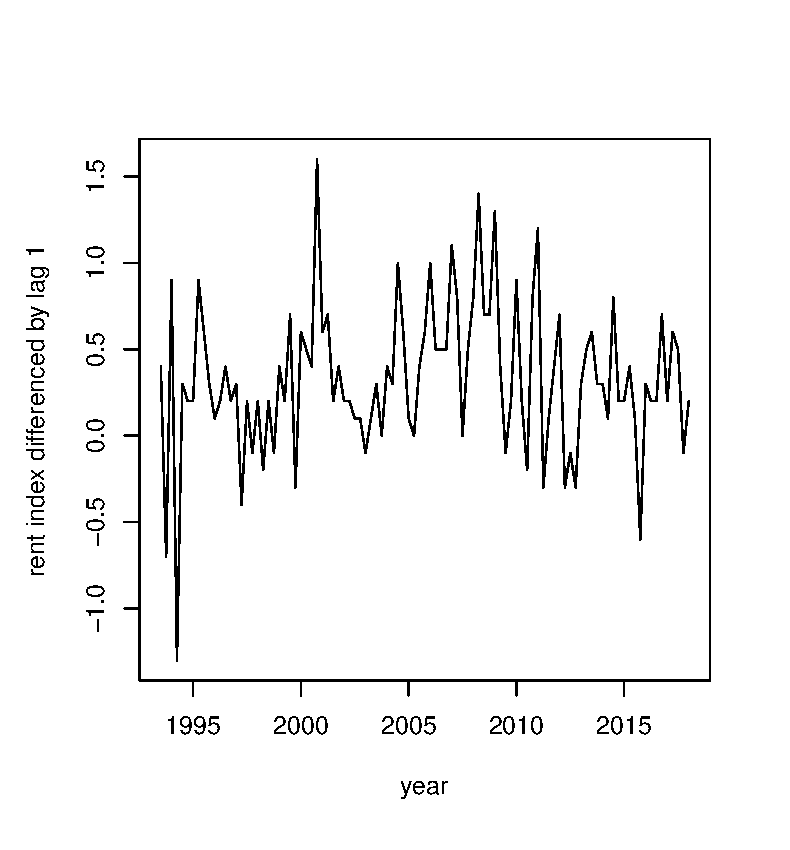
\includegraphics[angle=0,
width=0.5\textwidth]{diff1_timeseries}
\caption{once-differenced rent index
\label{fig:diff1_timeseries}}
\end{figure}
\begin{figure}
\centering
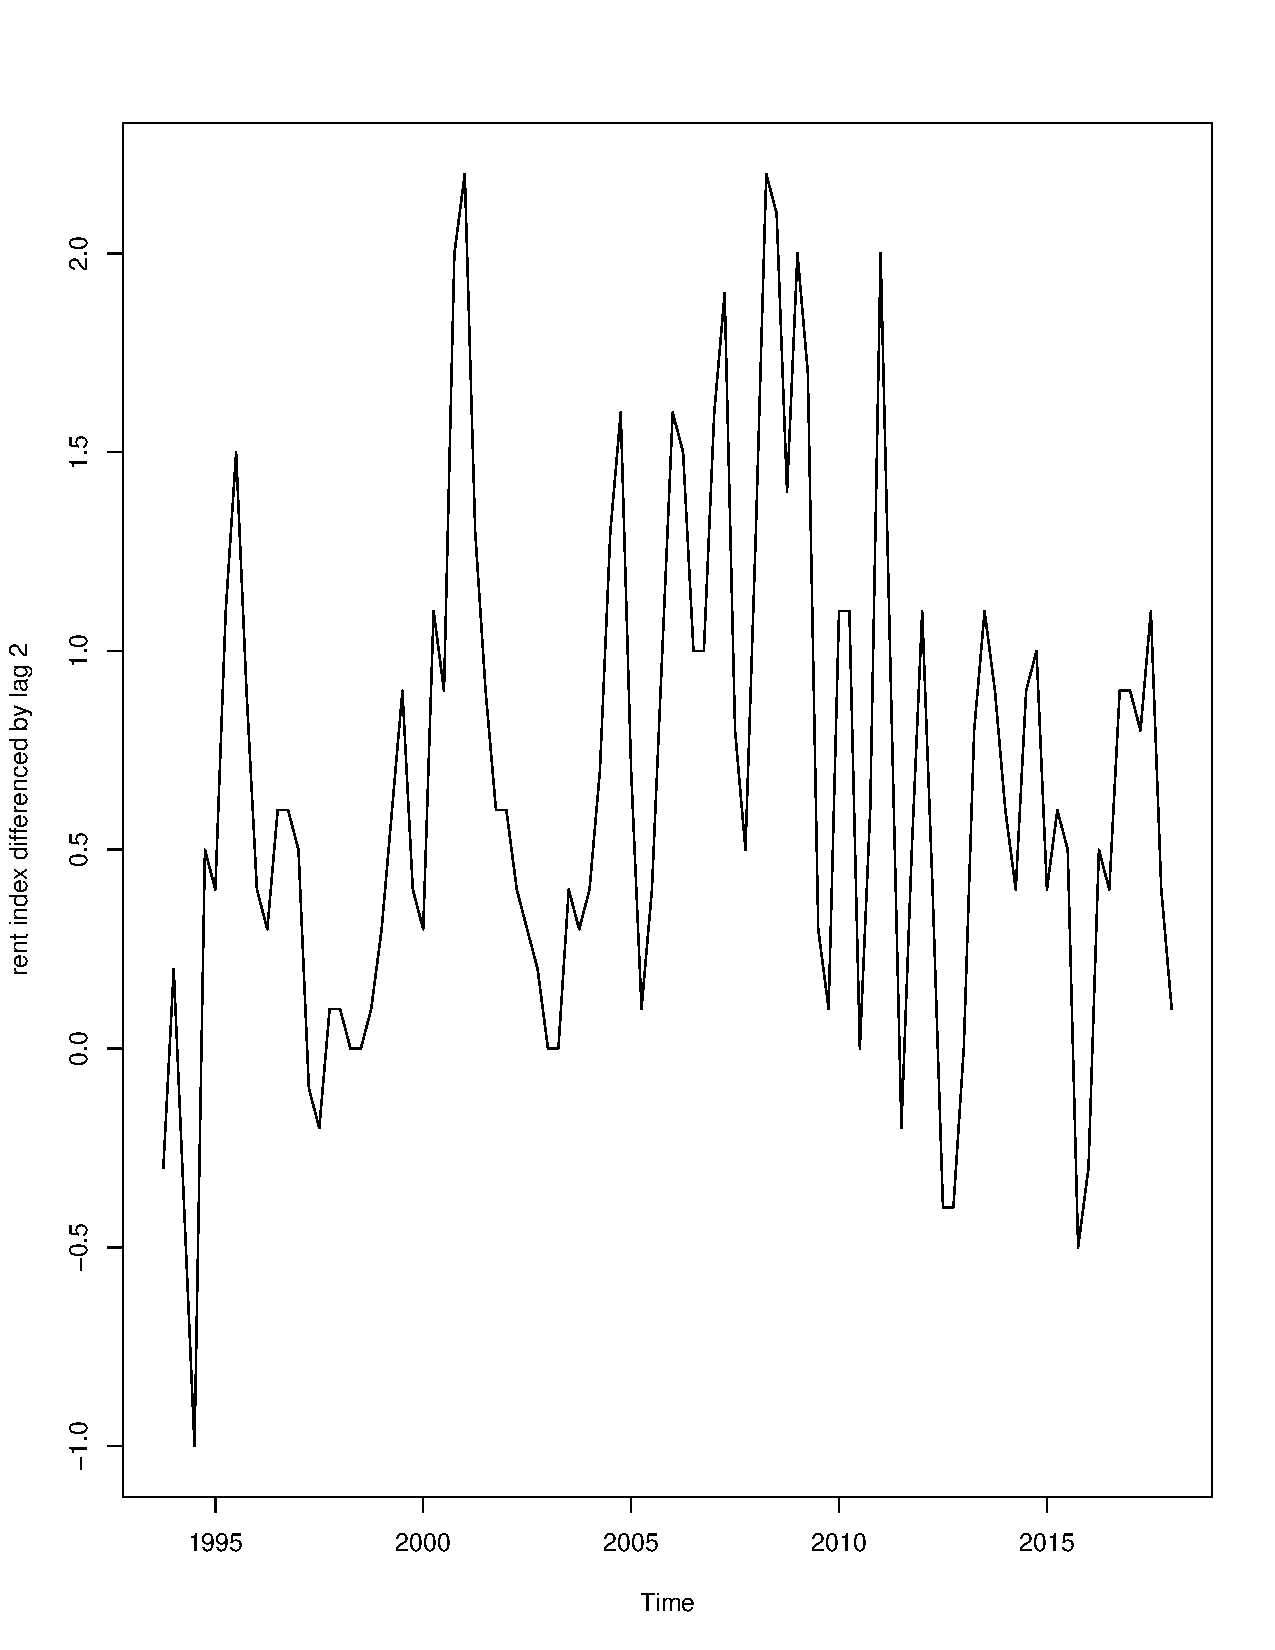
\includegraphics[angle=0,
width=0.5\textwidth]{diff2_timeseries}
\caption{twice-differenced rent index
\label{fig:diff2_timeseries}}
\end{figure}
\begin{figure}
\centering
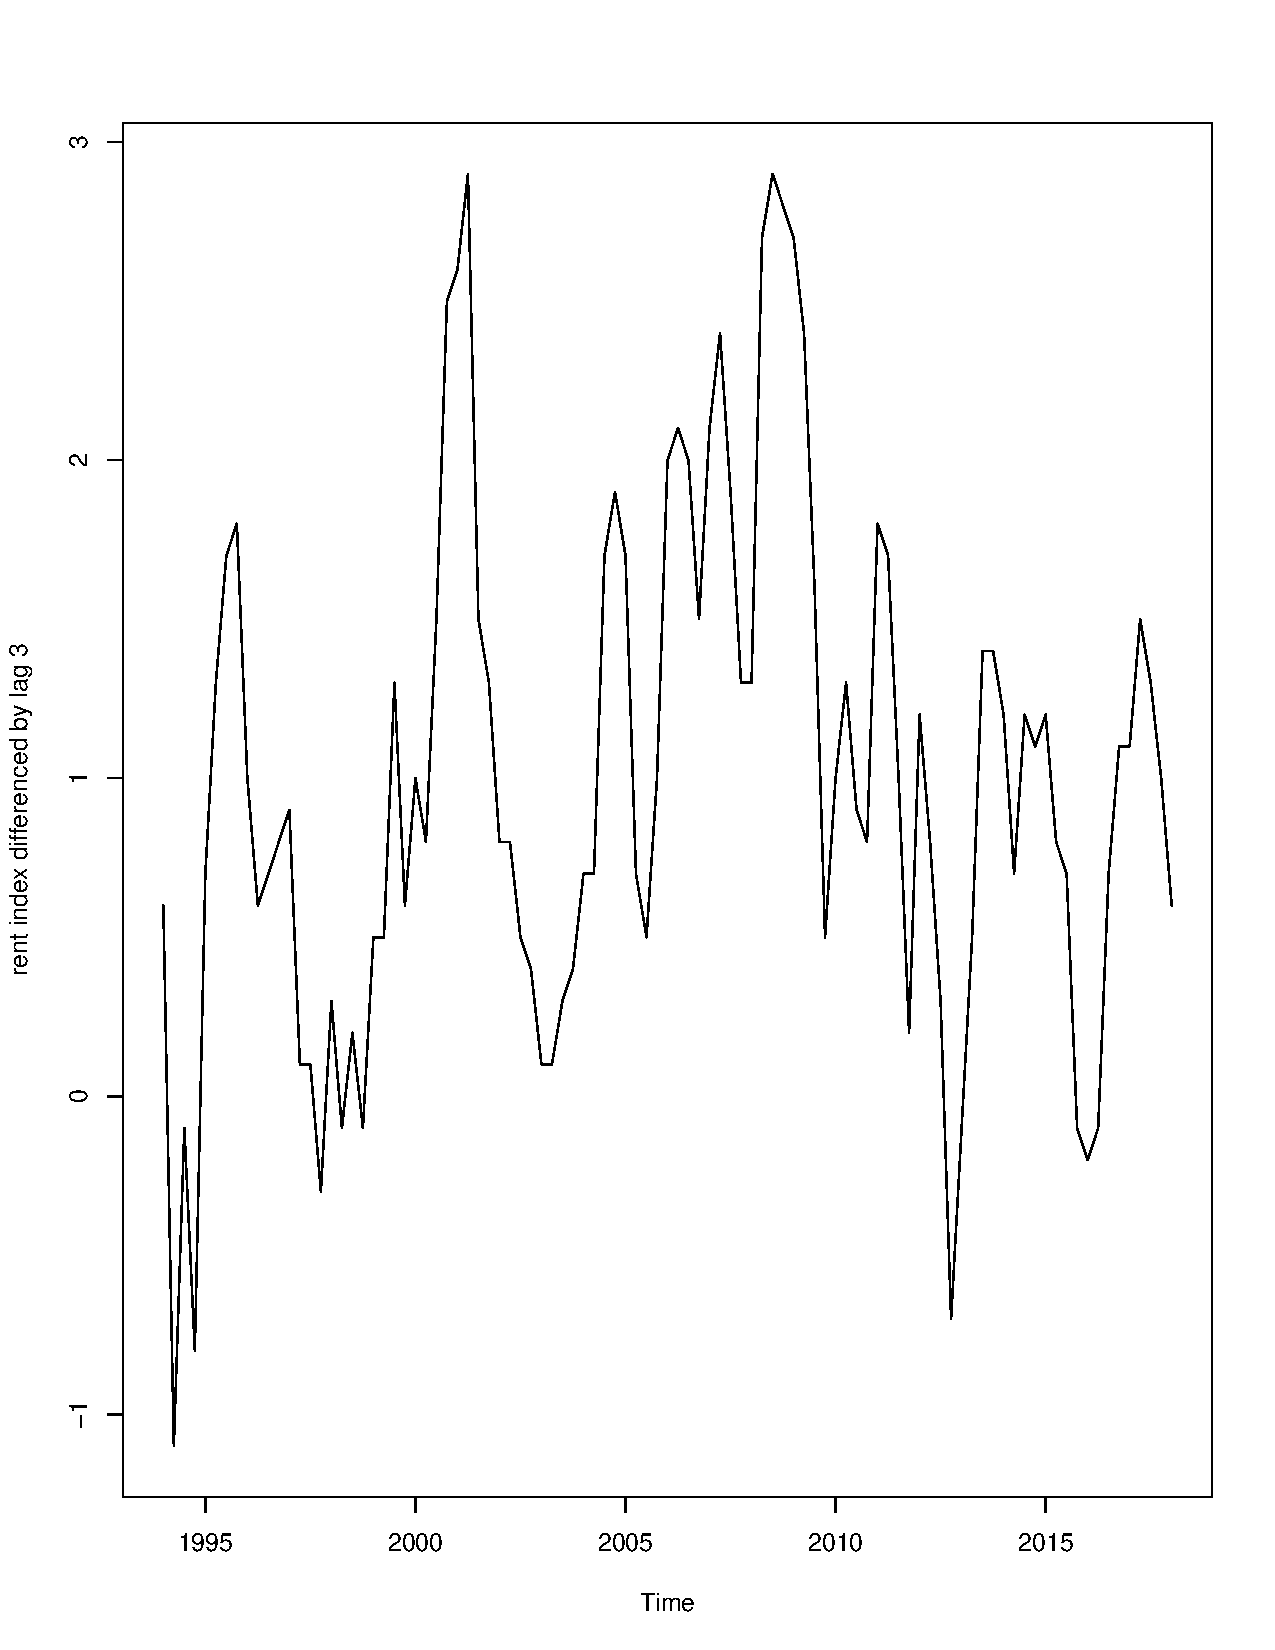
\includegraphics[angle=0,
width=0.5\textwidth]{diff3_timeseries}
\caption{triple-differenced rent index
\label{fig:diff3_timeseries}}
\end{figure}
\begin{figure}
\centering
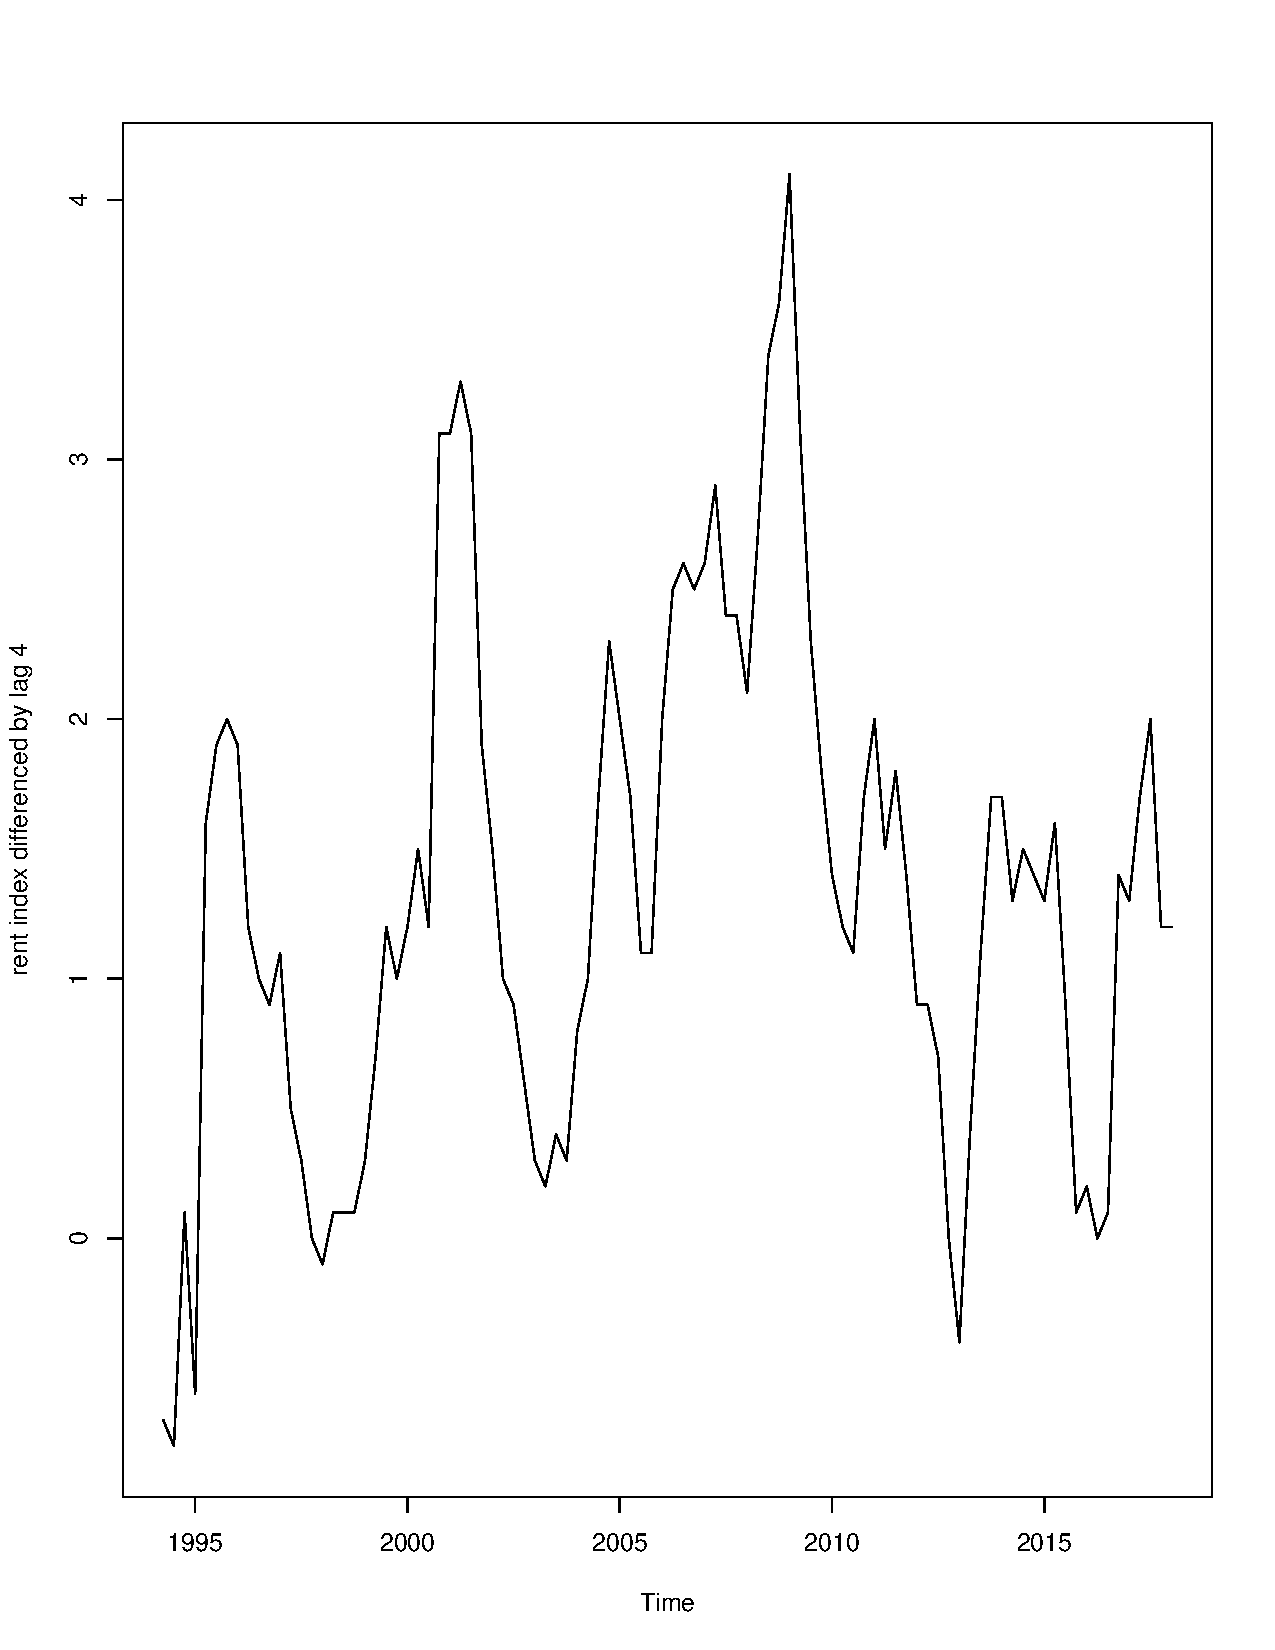
\includegraphics[angle=0,
width=0.5\textwidth]{diff4_timeseries}
\caption{quadruple-differenced rent index
\label{fig:diff4_timeseries}}
\end{figure}
For the first two models we were succesfully able to generate stationary residuals which don't depend on time. However figure~\ref{fig:diff1_timeseries} shows mostly patterns of a white noise which is not what we intended since in case of a white-noise-process prediction quality is poor (Expectation of $x_n+1$ would be 0 in case of a mean-centered series). This white-noise patterns is as well indicated by the sample autocorrelation function of the once-differenced series where all lags up to 40 fall well within the bounds of $+/-1.96sqrt{98}$ (brooks davis p.39)  (see figure~\ref{fig:diff1_acf}) . 
\begin{figure}
\centering
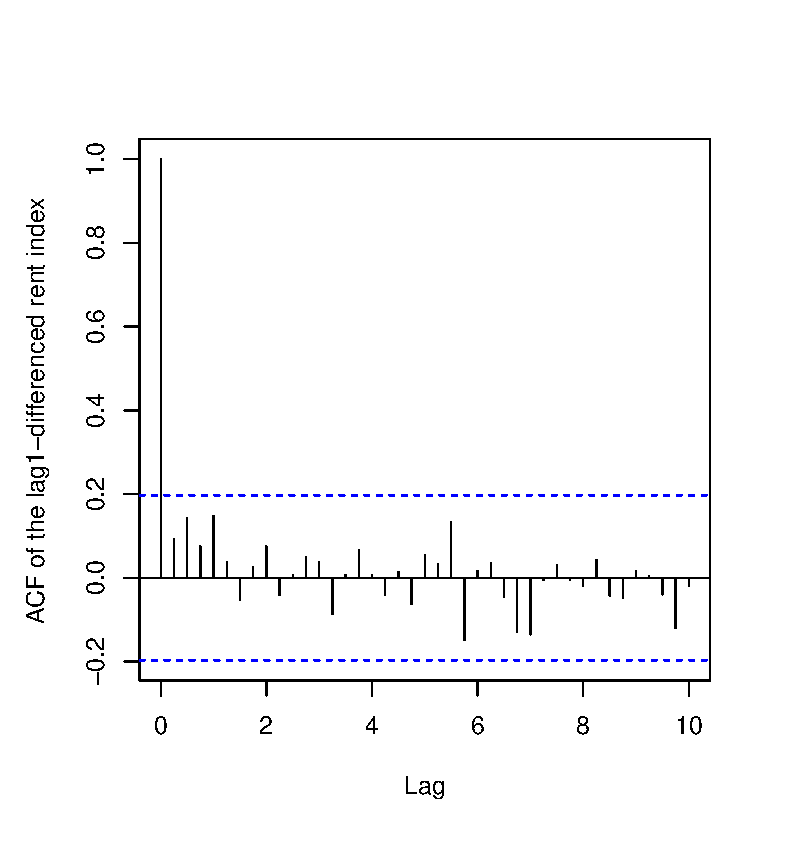
\includegraphics[angle=0,
width=0.5\textwidth]{diff1_acf}
\caption{auto-correlation function of the once-differenced series
\label{fig:diff1_acf}}
\end{figure}
The Ljung-Box-Test (Ljung-Box 1978, see brooks davis p. 36) indicates a p-value of 0.35, meaning that we cannot reject the iid-Hypothesis $H_0$ that there is independence between the observations. Therefore The Ljung-Box-Test emphasizes furthermore the independence of the values and the white-noise-patterns of the once-differenced series. Since white-noise would mean E0 and Variance sigma no more modelling would be necessary. 

\subsubsection{Diagnostics of the twice-differenced series}
\begin{figure}
\centering
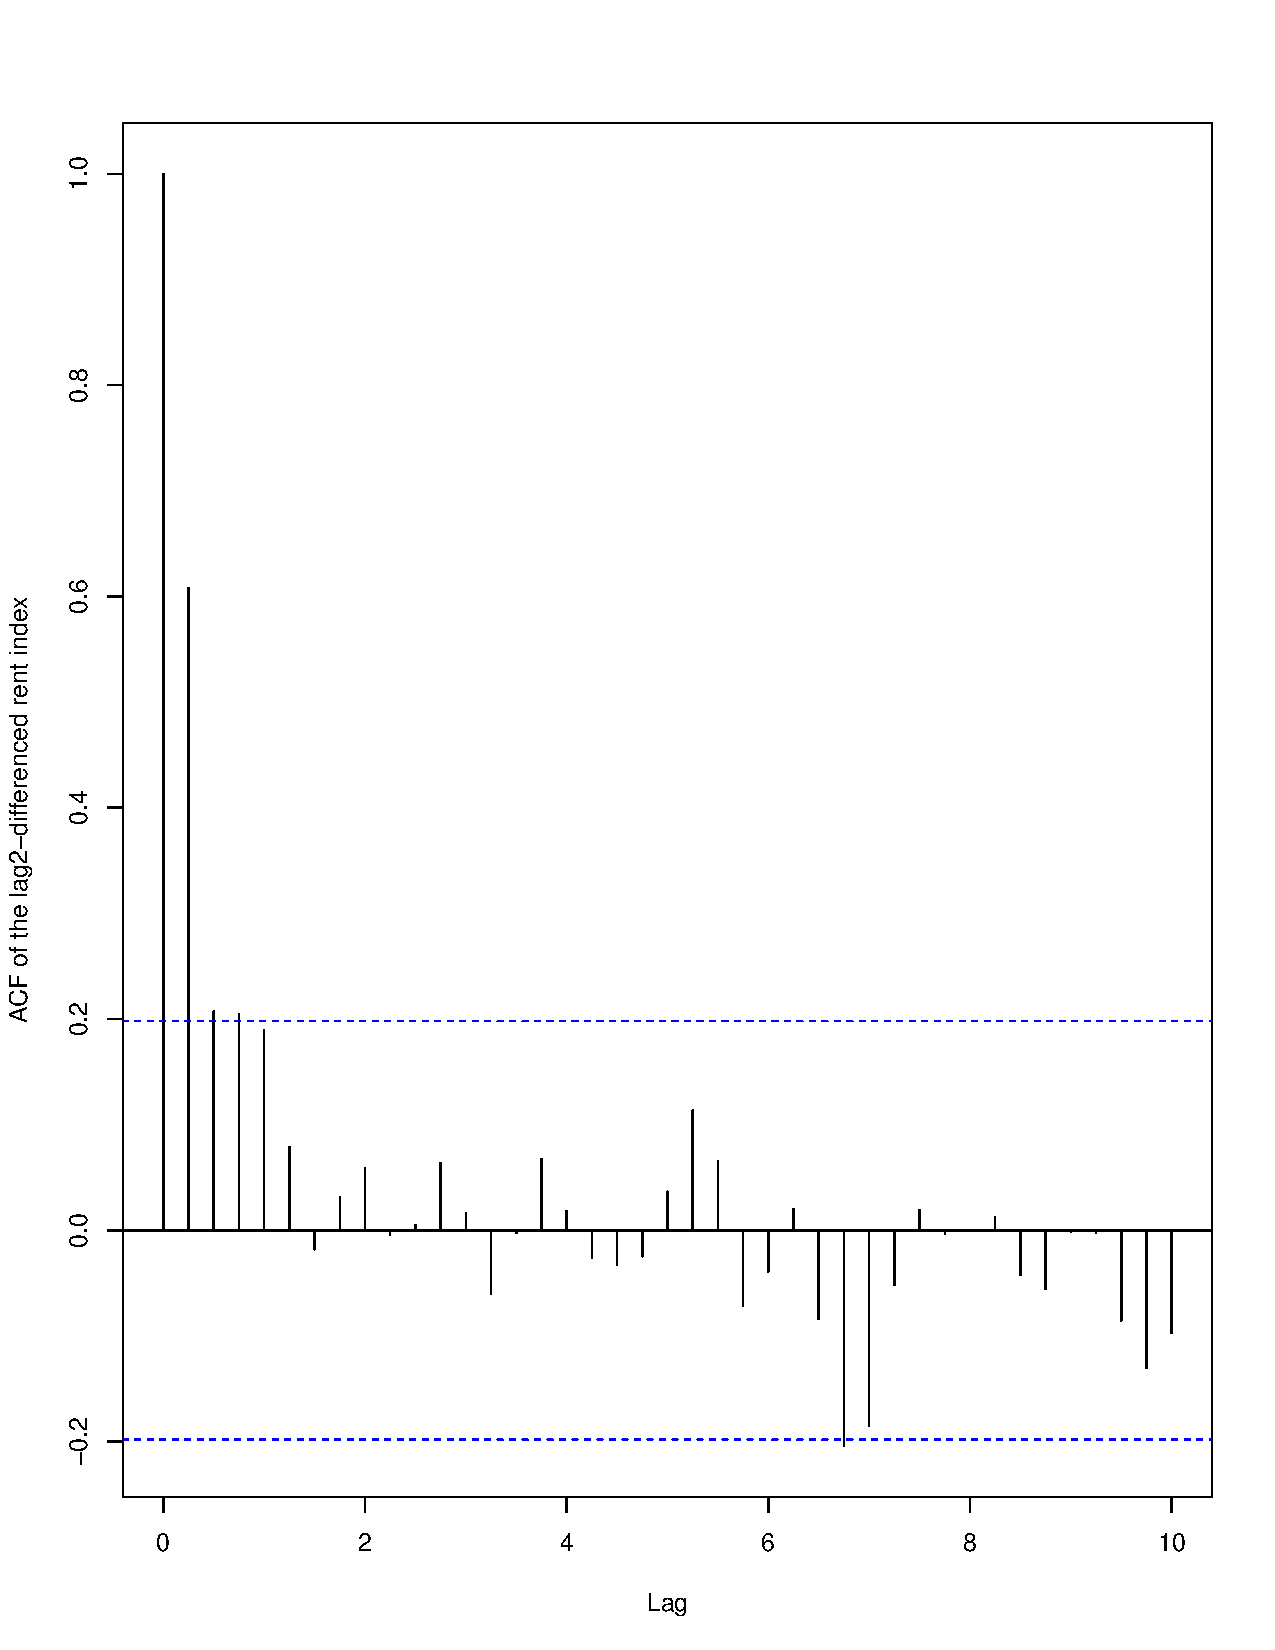
\includegraphics[angle=0,
width=0.5\textwidth]{diff2_acf}
\caption{auto-correlation function of the once-differenced series
\label{fig:diff2_acf}}
\end{figure}
\begin{figure}
\centering
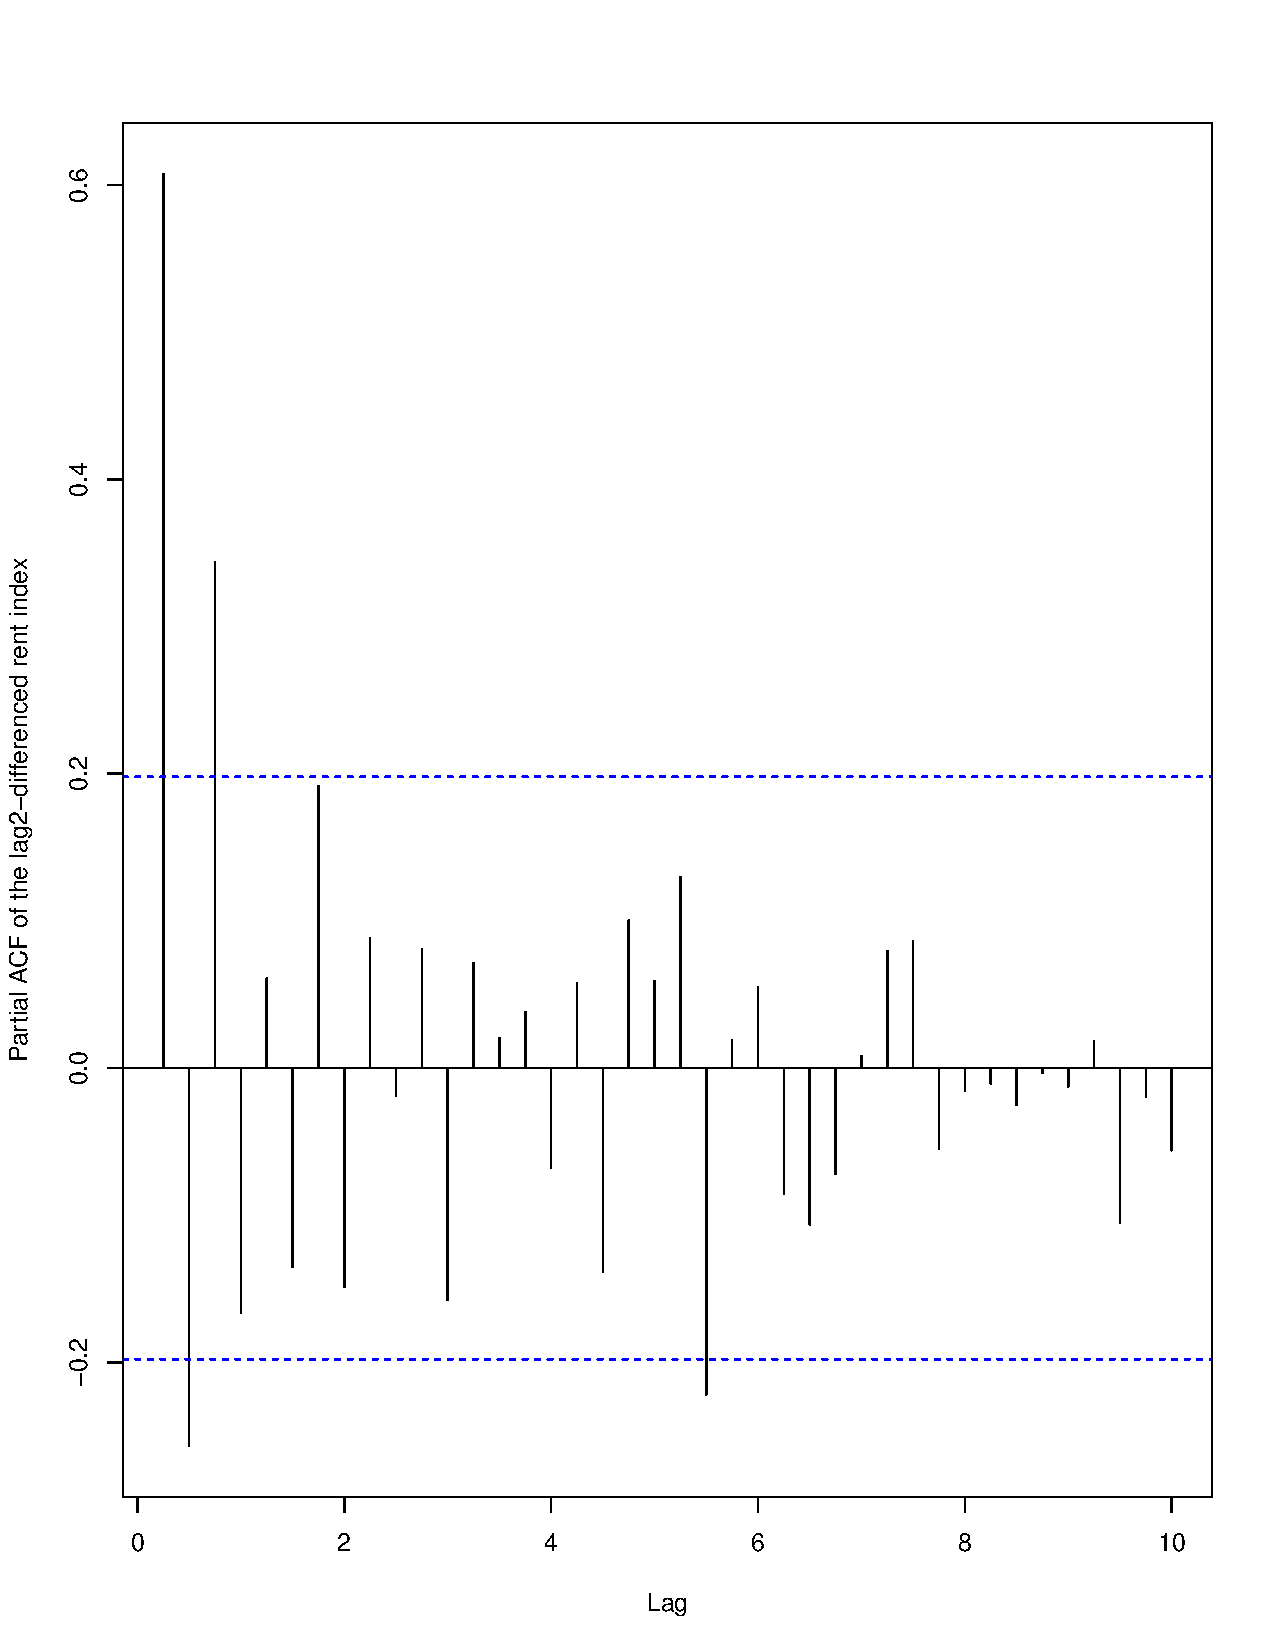
\includegraphics[angle=0,
width=0.5\textwidth]{diff2_pacf}
\caption{auto-correlation function of the once-differenced series
\label{fig:diff2_pacf}}
\end{figure}
In order to get better predictions and forecasting power than with pure white-noise-residuals seen in the once-differenced series, we now go for a twice-differenced model. Indeed our twice-differenced model doesn't show anymore iid-noisy patterns, indicating by the sample ACF (see figure~\ref{fig:diff2_acf} which shows at least a correlation at lag1 and some other lags are touching the $+/-1.96sqrt{n=100}$ - 95percent-confidence-bounds. The ACF of the twice-differenced model shows only a few significant lags which die out quickly. This is a good sign, meaning that on one hand we have correlations which are needed to do prediction on the other hand the covariance is not too large to be time-dependant and therefore we can conclude our series is stationary.
Cross-validation with a test data set considering only the last 35 of the 100 observations (see figure~\ref{fig:diff2_testset} above) confirms furthermore the non-stationary character of the twice-differenced-model 
Box.test(d2.indiceloyers.test, lag=2, type="Ljung-Box") p-value of 0.033 suggests the data are (time-)independent
adf.test(d2.indiceloyers.test, alternative = "stationary", k=2)  H0 of non-stationarity cannot be rejected which is not a problem, that could be due to lack of observations
kpss.test(d2.indiceloyers.test)  with a p-value>0.05 the test data seems to be stationary aswell
the data of the first segment's (1993 to 2009) twice-differenced series show independent observations as well (see figure~\ref{fig:diff2_trainingset}), however we can see a slightly slower increase in the segment from 2009 to 2018 indicating that in the years from 1993 to 2009 the growth in rental prices was higher than in the years in the second's segment which begins from 2009. that can be explained by the big baisse in the early 90ies, starting from a lower initial point and better conjunctural perspectives the increase was stronger, whilst from 2009 on the growth in rental prices slowed down, which can be very well explained by the US subprime crises beginning in the year 2008 followed by a long-taking global recession.
\begin{figure}
\centering
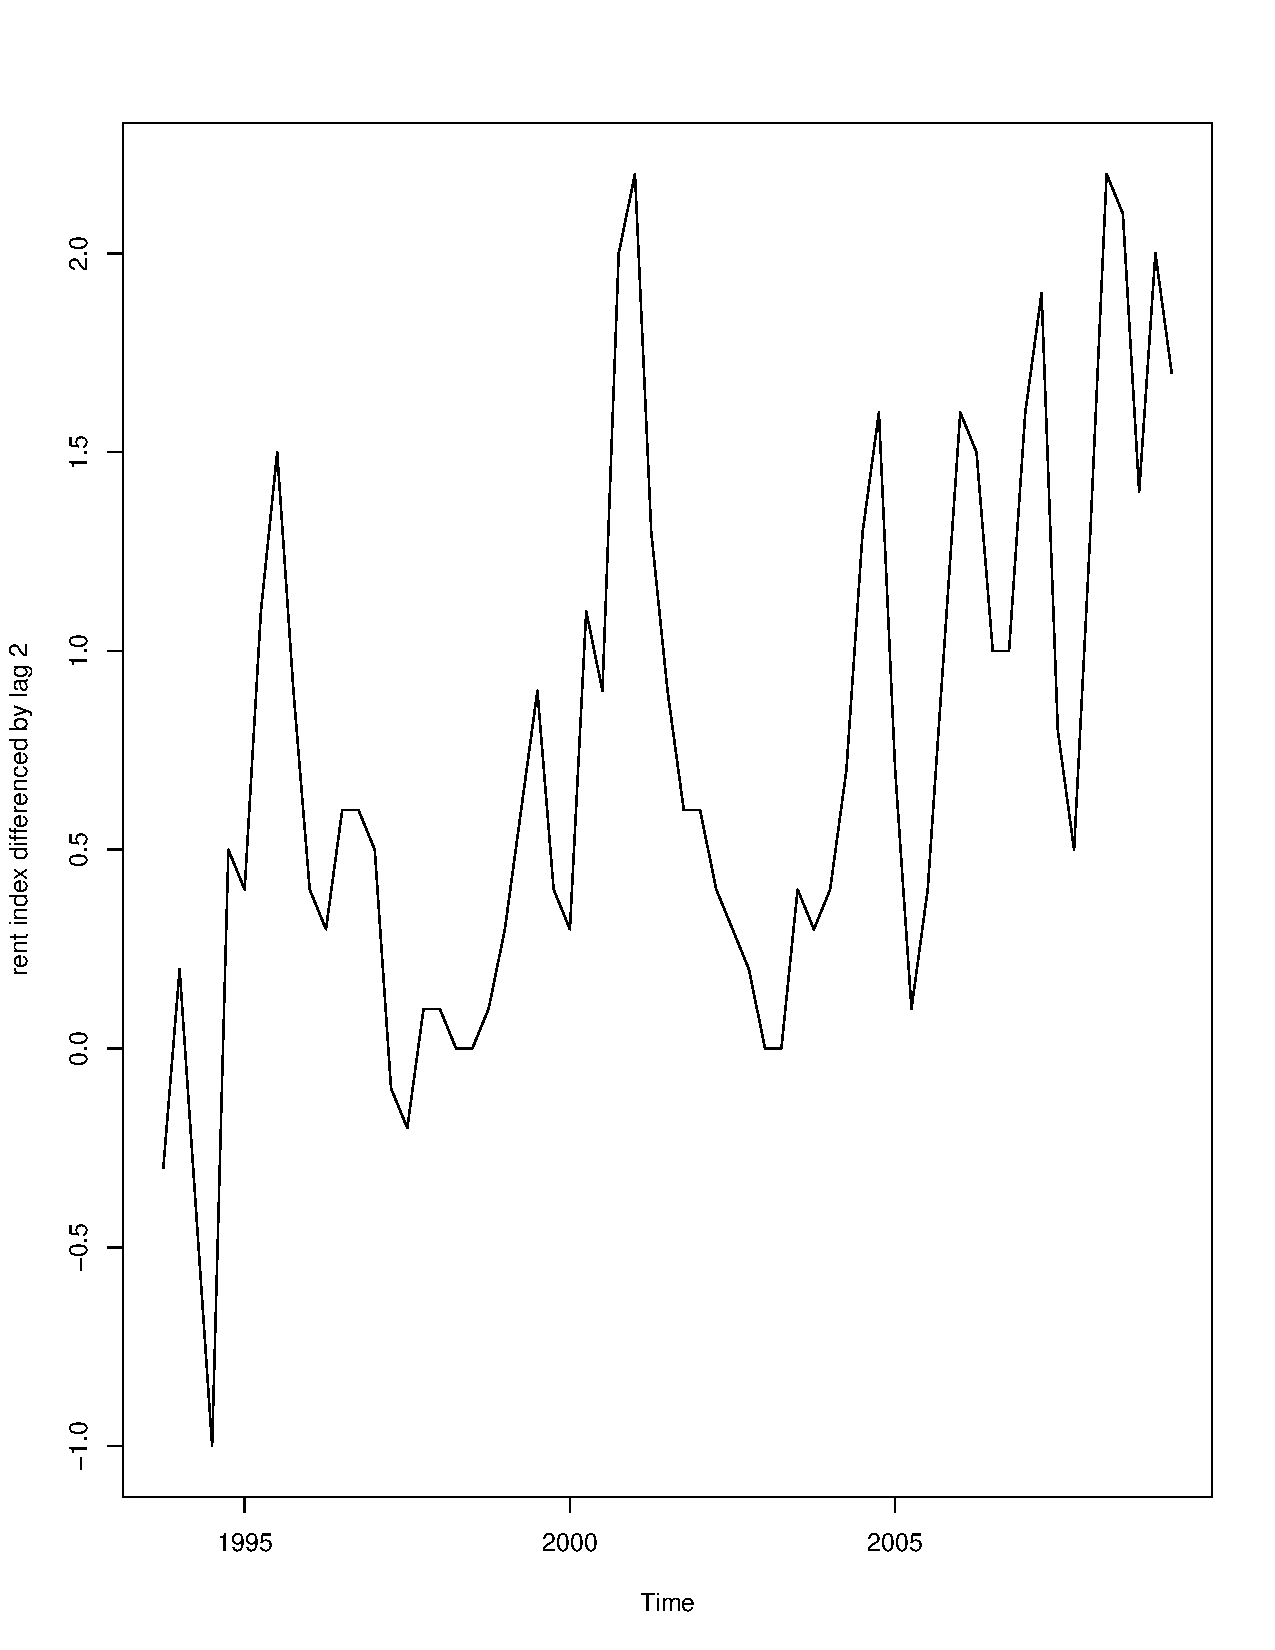
\includegraphics[angle=0,
width=0.5\textwidth]{diff2_trainingset}
\caption{twice-differenced series from 1993 to 2009
\label{fig:diff2_trainingset}}
\end{figure}
\begin{figure}
\centering
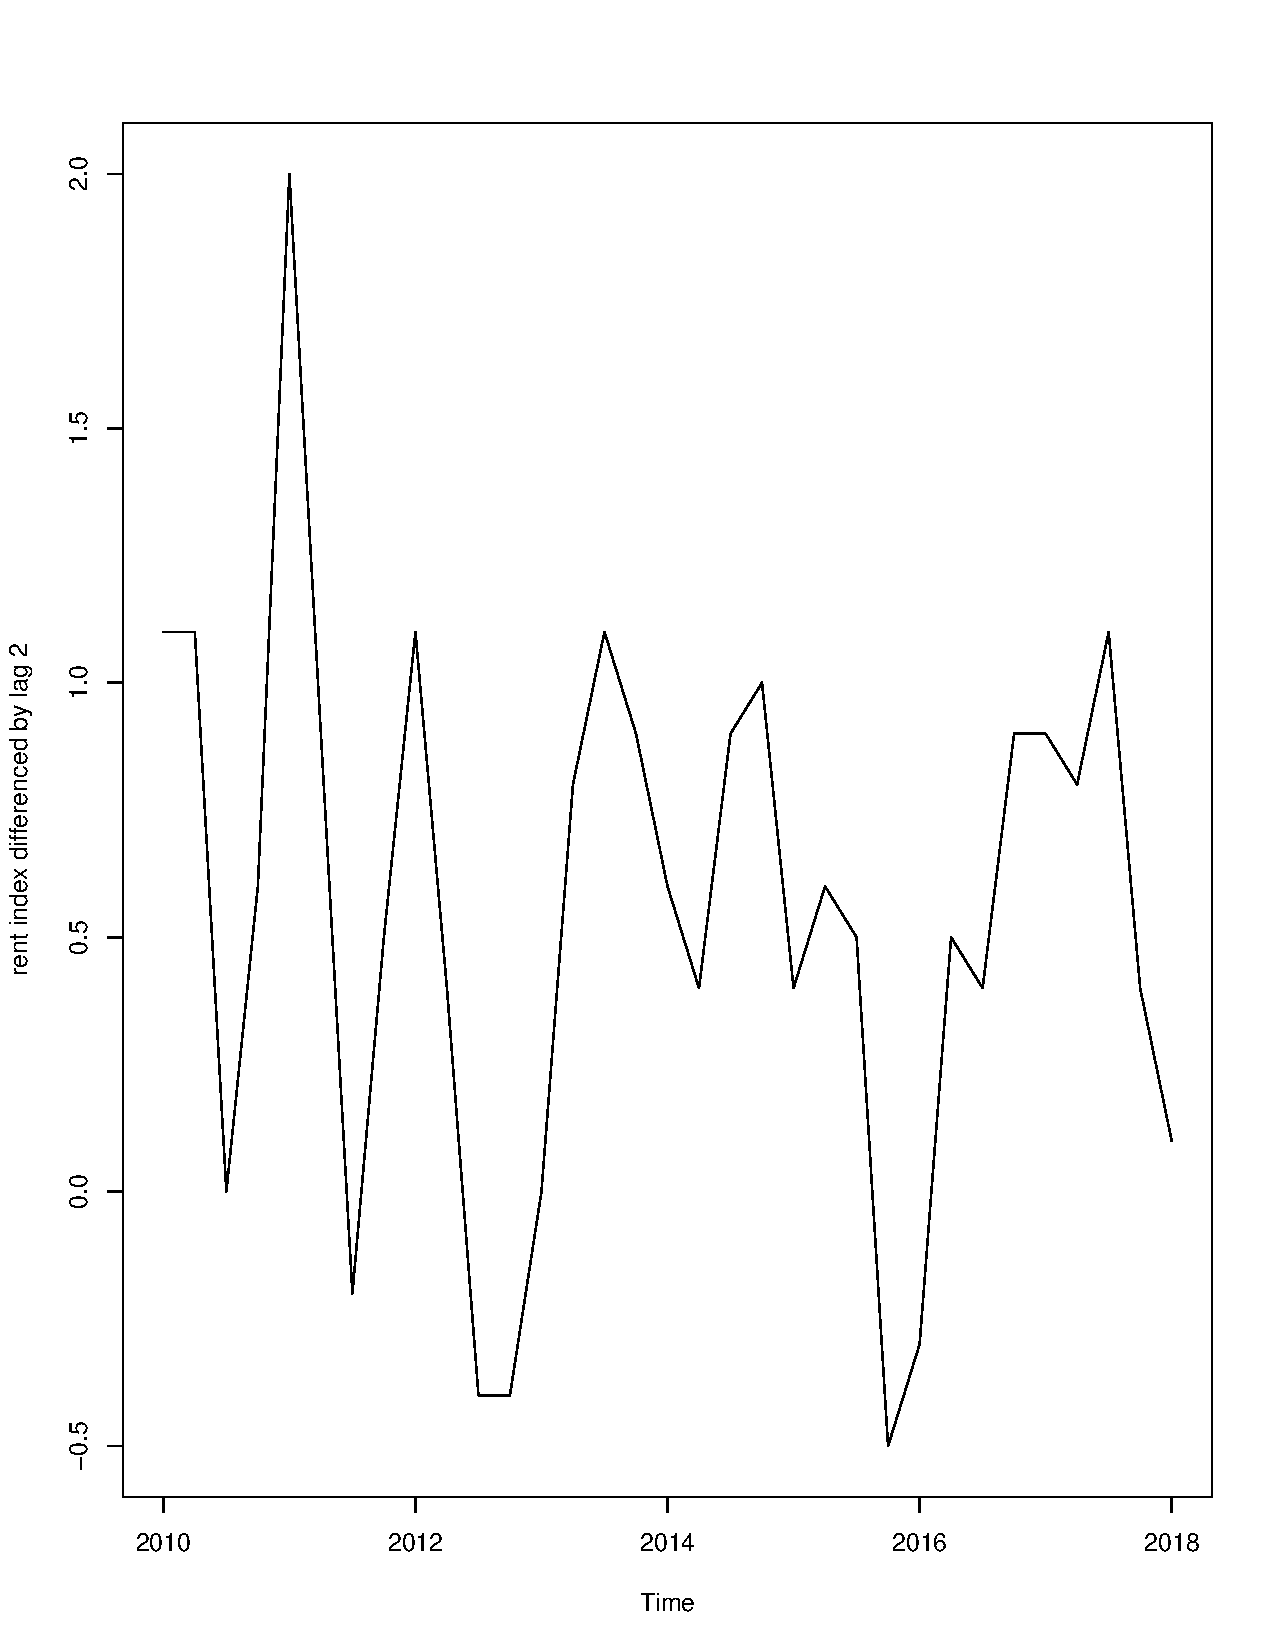
\includegraphics[angle=0,
width=0.5\textwidth]{diff2_testset}
\caption{twice-differenced series from 2009 to 2018
\label{fig:diff2_testset}}
\end{figure} 

\subsubsection{Diagnostics of the triple-/quadruple-differenced series}
Differencing by lag 3 and 4 is not appropriate neither since there is too much autocorrelation showed by the ACF a lot of bars outside the $+/-1.96sqrt{98}$ - bounds.


\section{Fitting and Testing the Model}

\begin{figure}
\centering
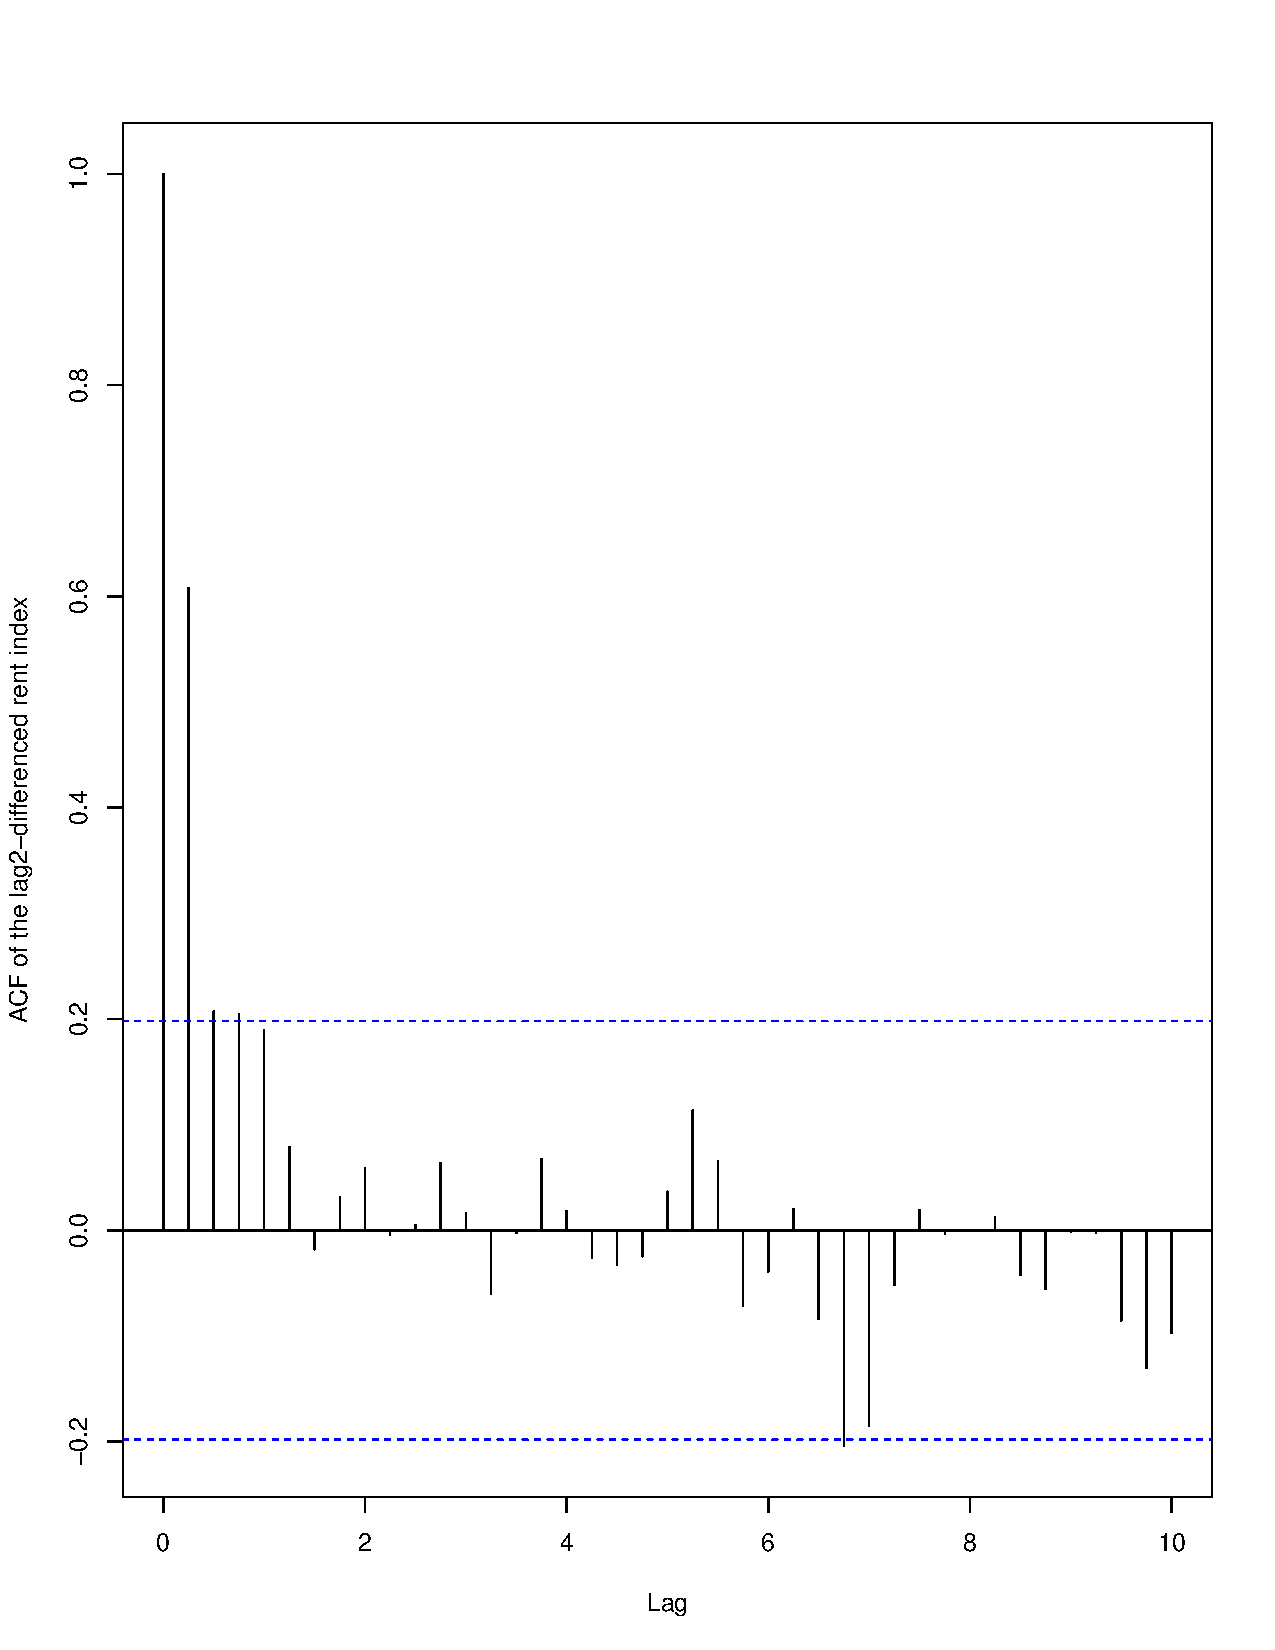
\includegraphics[angle=0,
width=0.5\textwidth]{diff2_acf}
\caption{ACF of the twice-differenced series
\label{fig:diff2_acf}}
\end{figure}
\begin{figure}
\centering
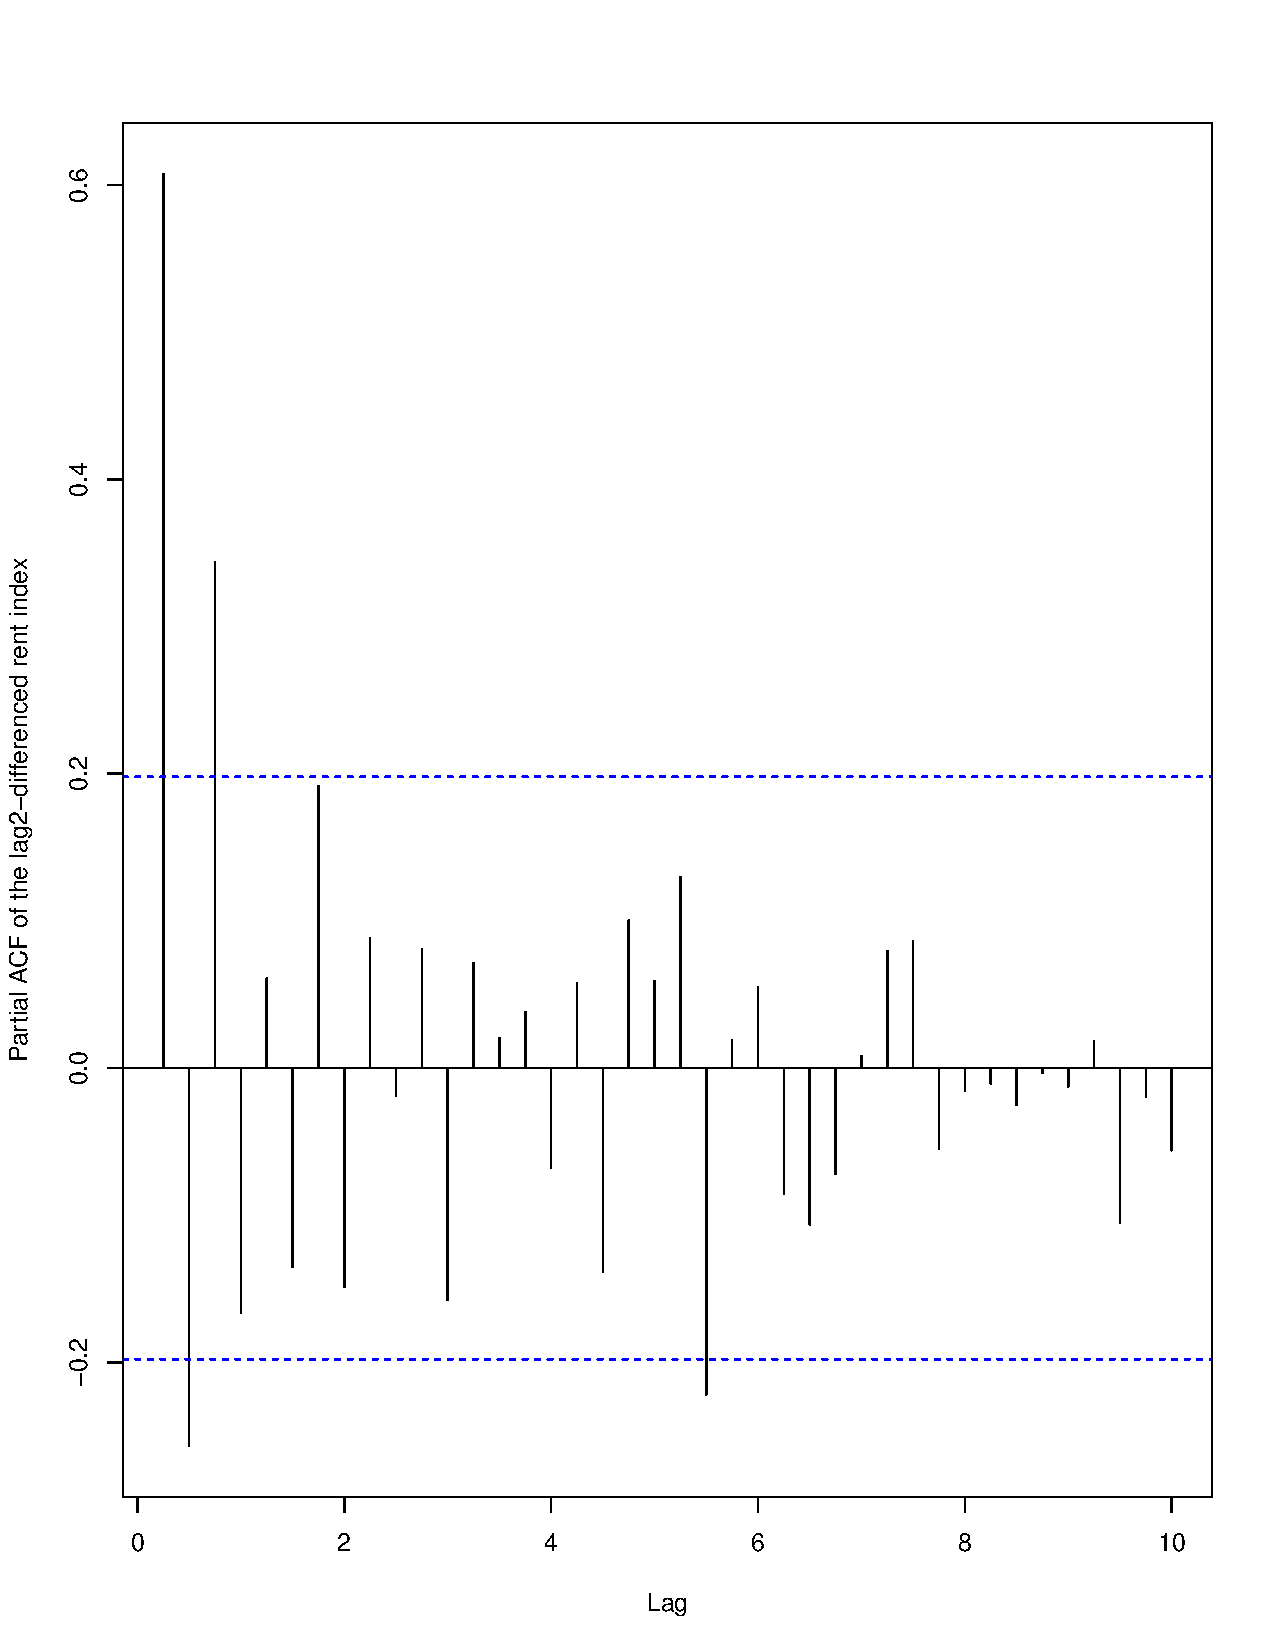
\includegraphics[angle=0,
width=0.5\textwidth]{diff2_pacf}
\caption{Partial ACF of the twice-differenced series
\label{fig:diff2_pacf}}
\end{figure}
from L6/7 p. 25. 
Therefore our model to rely on in order to transform our data into a stationary series should be the twice-differenced series, since the once-differenced series is too white-noisy and the triple/quadruple-differenced series show too large covariances (time-dependence/nonstationarity). From the visualization of the sample ACF and sample PACF of the twice-differenced series (see figure~\ref{fig:diff2_acf} and figure~\ref{fig:diff2_pacf},respectively) we can guess an AR(1) model as a suitable model for our data, since the ACF-plot shows only the first bar outside the borders (besides the following three touching them which we consider to give us to less evidence to justify an AR-model of order more than 1.
Our sample PACF ahat (h) is significantly different than zero for all h smaller or equal than 2 and becomes negligible for h larger than 2. indicating that a suitable model for the could be p=2 so an AR(2) rpocess. . This is further emphasized by the plot where the sample PACF values beyond lag 2 are approximately i.i.d. with a N(0,1/n) distribution. Therefore in our supposed AR(2) process rouglhly 95 percent of the sample PACF values beyond lag 2 should be within the bound +/- 1.96/sqrt(n) which is in fact true according to the plot (no single bar after p=2 is outside the bound +/-1.96/sqrt(n). sample PACF satisfyise |alpha(h)|>1.96/sqrt(n) for h<=p and |alpha(h)| < 1.06/sqrt(n) for h>p, which suggest an AR(p=2) model for our data.
in other words: The fact that all of the PACF values beyond lag 3 fall within the bounds suggests the possible suitability of an AR(p=3) model for the mean corrected data set Xt=St-46.93. One simple way to estimate the parameters phi1 phi2 phi33 and sigma2 of such a model is to require tha the ACVF of the model at lags 0,1 and 2 should match the sample ACVF at those lags. Substituting the sample ACVF vlaues gammahat0 gammahat1 gammahat2 for gammma0 gamma1 and gamma 2 in the first thee equations of (3.2.5) and (3.2.6) and solving for phi1 phi2 phi3 and sigma2 gives the fitted model Xt-1.318xt-1+255Xtte-2+sxt-3=Zt wit hZt  WN (this method of model fitting is called yule-walker estimation ) (brock davis p. 99)

Furthermore the choice of an AR(p) model is underlined by the fact that the ACF plot shows an exponentially decreasing patterns of |rho(h)| and PACF patterns with p=3 "spikes". Exponentially decrease in AR and alpha(h)=0 for h>p=3 in PACF are typical properties for an AR(p)-process.

In addition to the visualised evidence provided above further analytical evidence for an AR(1)-process is provided by the preliminary prediction by using the Yule-Walker-Algorithm for estimating roughly the AR-coefficients (phi). As we can see in table xy only the first estimated coefficient is a strong coefficient, all the others are close to zero and therefore not significant, emphasizing our assumption to go on with an AR(1)-Model.
The program used from the ITSMR package will search thorugh all the Yule-Walker AR(p) models, p=0,1,....,27, selecting the one with smallest AICC value. (explain AICC, corrected AIC) The minimum-AICC Yule-Walker AR model turns out to be the one defined by (eq 5.1.14) with p=1 and AICC value 74.541

In addition the estimated coefficient by Yule-Walker-Algorithm guarantees us that our model is causal. We can see that aswell in table x which shows indicating that the unit root is (slightly) outside the unit circle, with an value of 1.023714.

causality of a process (brock davis p. 85)

HannanRissanen-Algoritm shows strongly varying coefficients theta (q) for different fixed numbers of coefficients
which further underlines our assumption that an AR(p)-model suits our data well instead of an MA(q) or ARMA(p,q) process.


BrockwellDavis p. 193 a root near 1 of the autoregressive polynomial suggests that the data should be differenced before fitting an AMA model, whereas a root near 1 of the moving-average polynomial indicates that the data were overdifferenced. 

\section{Prediction of future values}

\section{Discussion}
Discuss your results, the strengths and the limitations of your own analysis. 

\section{Conclusion}
Conclude the report. Sketch further analyses that you could carry out if you would have more time.


\section{quotation examples}
Hello World. Mister Resnick wrote a beautiful book about Harry, see \citep{Resnick92}. If you want something more fancy, try \citet{Baddeley07}.
\\By looking at the plot we cannot definitely exclude that there might exist some seasonal patterns. To detect if a seasonality effect is really present in the series, we test it by modelling the seasonality and add it in the linear model. 


\begin{figure}
\centering
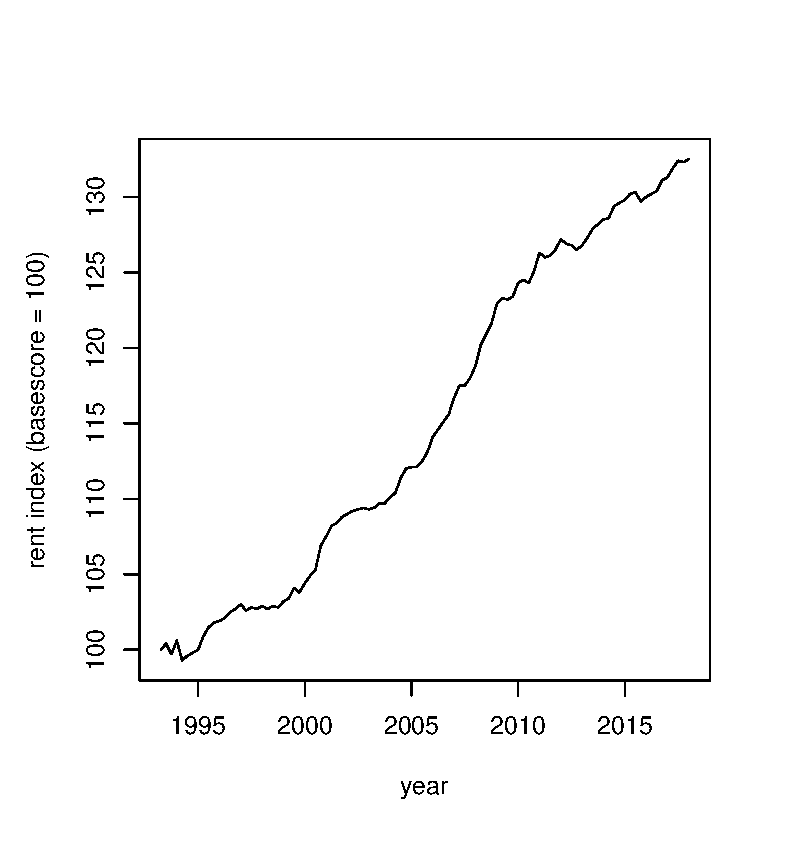
\includegraphics[angle=0,
width=0.5\textwidth]{indiceloyers_timeseries}
\caption{This is a test.}
\end{figure}
\bibliography{Bibliography}
\bibliographystyle{apa}
\end{document} 
